% Figure from MATH 556 notes, section 37. Compile with the notes preamble.
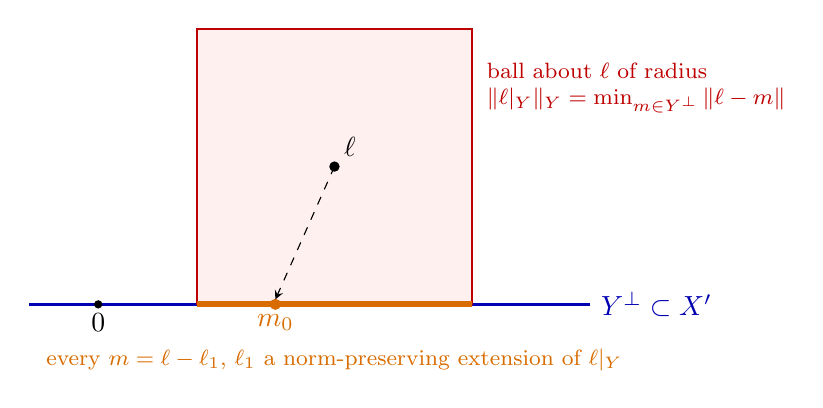
\begin{tikzpicture}[scale=1.25, >=stealth]
    \draw[very thick, blue!70!black] (-2.3,0) -- (3.4,0) node[right] {$Y^\perp \subset X'$};
    \fill (-1.6,0) circle (1.2pt) node[below] {$0$};
    \fill[red!6] (-0.6,0) rectangle (2.2,2.8);
    \draw[thick, red!75!black] (-0.6,0) rectangle (2.2,2.8);
    \draw[line width=2.2pt, orange!85!black] (-0.6,0) -- (2.2,0);
    \fill (0.8,1.4) circle (1.5pt) node[above right] {$\ell$};
    \fill[orange!85!black] (0.2,0) circle (1.6pt) node[below] {$m_0$};
    \draw[->, dashed] (0.8,1.4) -- (0.2,0.05);
    \node[right, align=left, font=\footnotesize, red!75!black] at (2.25,2.2) {ball about $\ell$ of radius\\ $\|\ell|_Y\|_Y = \min_{m \in Y^\perp} \|\ell - m\|$};
    \node[below, align=center, font=\footnotesize, orange!85!black] at (0.8,-0.35) {every $m = \ell - \ell_1$, $\ell_1$ a norm-preserving extension of $\ell|_Y$};
\end{tikzpicture}
